\section{Použité technologie}

\subsection{Python}

\begin{wrapfigure}{R}{0.5\textwidth}
 \centering
 \includesvg[width=0.5\textwidth]{images/python-logo}
 \caption{Logo programovacího jazyka Python}
\end{wrapfigure}

Python je moderní interpretovaný programovací jazyk, který byl navržen v roce 1991 nizozemským programátorem Guido van Rossumem. Nabízí rozličná programovací paradigma: imperativní, procedurální, funkcionální nebo objektově orientované, které jsem ve své práci použil nejčastěji.

Python je vyvíjen jako open source projekt, jeho zdrojové kódy jsou tedy veřejné a je možné do nich přispět. Jeho výchozí implementace se nazývá \uv{CPython} dle jazyka C, ve kterém je implementována. Mezi další jeho alternativní implementace patří \uv{Jython} naprogramovaný v jazyce Java nebo \uv{IronPython} v prostředích .NET a Mono.

Jednou z velkých výhod Pythonu je jeho rozšířitelnost. Oficiální portál pro rozšiřující balíčky \href{https:\/\/pypi.python.org\/pypi}{PyPi} aktuálně nabízí okolo 74 tisíc knihoven. Kterýkoliv z těchto balíčků je možno pomocí nástroje pip nainstalovat a používat. Jednou z dalších možností, jak rozšířit jeho funkčnost, je naprogramovat si vlastní rozšíření v jazyce C.

Python je aktuálně vyvíjen ve dvou hlavních větvích; větvi Pythonu verze 2 a verze 3. Motivace pro vydání verze 3 byla především ve sjednocení práce s řetězci (Python verze 2 rozlišoval řetězce ASCII znaků a řetězce Unicode znaků), celočíselného dělení a některých syntaktických vylepšení jazyka. Poslední vydaná verze Pythonu je 3.5 a její hlavní výhodou je přidání podpory pro asynchronní volání funkcí a podpory pro typovost parametrů a návratových hodnot funkcí a metod.

\subsubsection{Jednotkové testování}

Jednotkové automatické testování je jeden z způsobů, jak vývojáři ulehčit úpravu, vytváření i mazání částí zdrojových kódů. Jednotka testu je v množina asercí (předpokladů), které kontrolují vývojářem vytvořené modelové situace nad zdrojovým kódem programu. Automatické testování je poté automatické spouštění testů např. po změně zdrojového kódu a určení, zda testy prošly korektně (aserce všech testů jsou pravdivé). Samotný test je však psán samotným vývojářem, což při testování může vytvářet klamný dojem \uv{bezchybnosti} zdrojového kódu aplikace, protože vývojář jakožto člověk, je bytost chybující a samotný kód testů může být napsat chybně a aserce jsou v tu chvíli bezpředmětné, protože jsou např. vždy pravdivé a znehodnocují tím korektnost a správnost testů projektu.

Níže je uveden příklad třídy k testování. Třída \ic-MathOperations- je určena k základním matematickým operacím, pro názornost pro sčítání a dělení. 
\begin{lstlisting}[caption={Příklad třídy MathOperations k testování}]
class MathOperations(object):
	@staticmethod
	def add(a, b):
		return a + b

	@staticmethod
	def divide(a, b):
		return a / b
\end{lstlisting}

\begin{sloppypar}
	Pomocí volání \ic|MathOperations.add(40, 2)| získáme \ic|42|, resp. při \ic|MathOperations.divide(36, 6)| je výsledkem \ic|6|. Ve své práci používám balíček pro testování \ic|unittest| dodávaný přímo s programovacím jazykem Python. Jako hlavní nástroj pro jednotkové testování nabízí tento balíček třídu \ic|TestCase|, která obsahuje celou řadu metod pro testování asercí (\ic|assertEqual|, \ic|assertTrue|, \ic|assertEqual|, \ic|assertIn|, \ic|assertIs| nebo i komplexnější jako \ic|assertDictEqual|, \ic|assertRegex| nebo \ic|assertDictContainsSubset|) a potomky této třídy je potom možno automaticky spouštět a vyhodnocovat. Tyto předpoklady tedy zapíšeme jako metody do obalující třídy:
\end{sloppypar}

\begin{lstlisting}[caption={Základní TestCase pro třídu MathOperations}]
class TestMathOperations(TestCase):
	def test_add(self):
		self.assertEqual(
			MathOperations.add(40, 2),
			42
		)

	def test_div(self):
		self.assertEqual(
			MathOperations.div(36, 6),
			6
		)
\end{lstlisting}

V případě spuštění a úspěšného otestování této třídy by byl výstup tento:
\begin{lstlisting}[language=bash, caption={Ukázka výstupu ze spuštění testů}]
test_add (TestMathOperations) ... ok
test_div (TestMathOperations) ... ok

------------------------------------
Ran 2 tests in 38ms

OK
\end{lstlisting}


{\itshape
	Ve své aplikaci používám vlastní poděděnou třídu \ic|TestCase|, protože pro každé pokročilejší testování pohledů frameworku Flask je nutné mít správně nakonfigurovaný objekt pro \uv{vnější} přístup ke serveru, a také kvůli zobecnění některých častých operací v mých testech - detaily ohledně testů jsou v sekci \fullref{sec:implementation}.
}


Poté ale může dojít k následující změně zdrojového k\'{o}du - vznikne požadavek na metodu \ic|MathOperations.add|, a to konkrétně na zvýšení počtu parametrů na tři. Ne ve všech případech se ovšem bude volat tato metoda i se třetím parametrem, musí být tedy zajištěna \textbf{zpětná kompatibilita}.
\begin{lstlisting}[caption={Vylepšená implementace metoda MathOperations.add}]
@staticmethod
def add(a, b, c=0):
	return a + b + c
\end{lstlisting}
Do metody testující sčítání je tedy nutné přidat aserci i pro tři parametry:
\begin{lstlisting}[caption={Testovací metody pro upravenou implementaci MathOperations.add}]
def test_add(self):
	self.assertEqual(
		MathOperations.add(40, 2),
		42
	)
	self.assertEqual(
		MathOperations.add(10, 7, 3),
		20
	)
\end{lstlisting}
Tímto testem máme potvrzenou korektní jak pro dvouparametrické volání, tak pro \uv{nové} tříparametrické volání. Podstata úprava zdrojového kódu tkví v zachování předchozích asercí - je tak zajištěna zpětná kompatibilita. Jako další požadavek na metodu \ic|MathOperations.add| může typicky přijít přidání dalšího parametru, kdy je vhodné vzhledem k aktuální implementaci metody \ic|add| tuto metodu přeimplementovat následovně:
\begin{lstlisting}[caption={Finální implementace metody MathOperations.add}]
@staticmethod
def add(*values):
	return sum(values)
\end{lstlisting}
\textit{
  Zápis \\ic|*values| je velmi specifický pro jazyk Python. 
}
A ke testovacím asercím přidat i jednu komplexnější obsahující volání s vytším počtem parametrů:
\begin{lstlisting}[caption={Finální test pro metody MathOperations.add}]
def test_add(self):
	...
	values = tuple(randint(0, 100) for _ in range(10))
	self.assertEqual(
		MathOperations.add(*values),
		sum(values)
	)
\end{lstlisting}
\subsection{Flask}

% \begin{figure}[H]
%  \centering
%  \includesvg[width=.3\textwidth]{images/flask-logo}
%  \caption{Logo webového frameworku Flask}
% \end{figure}

\begin{wrapfigure}{R}{\textwidth/3}
    \centering
    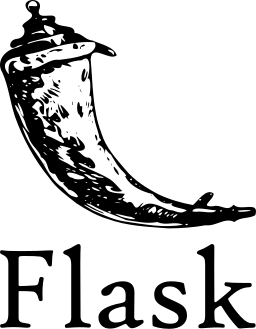
\includegraphics[width=\textwidth/3]{images/flask-logo}
    \caption{Logo webového frameworku Flask}
\end{wrapfigure}

Flask je webový framework implementovaný v jazyce Python. Mezi jeho přednosti patří vestavěný vývojářský server, plná podpora pro unit testování a kvalitní dokumentace. Vzhledem k jeho variabilitě a v základu tenké architektuře bylo nutné přidat abstraktní vrstvy pro samotné zpracování herních akcích a podobně.

Vzhledem k tomu, že je framework téměř stoprocentně pokryt testy, lze jednoduše usuzovat z těchto testů o funkčnostech frameworku a také je velmi snadné psát vlastní testy na kteroukoliv komponentu aplikace.

\subsection{HTTP}

HTTP (HyperText Transfer Protocol) je standardizovaný internetový protokol pro výměnu HTML kódu. Jeho první koncept vznikl v roce 1991 jako veze 0.9, o pět let později byla uvedena verze 1.1 a verze 1.1, která je používaná dodnes byla uvedena v červu roku 1999. V dnešní době je používán nejen k výměně HTML kódu, ale jeho rozšíření MIME \footnote{Multipurpose Internet Mail Extensions} poskytuje možnost přenosu souborů jakéhokoliv typu. Samotný HTTP nezajištuje zabezpečení ani integritu dat. Nadstavbu nad HTTP tvoří HTTPS, jehož komunikace je šifrována pomocí SSL nebo TLS.

HTTP pracuje na principu request-response (požadavek-odpověd). HTTP požadavek ve formě plaintextu je vyslán ze klientského zařízení, ten je serverem zpracován a nazpět jsou odeslány tzv. hlavičky odpovědi a poté i samotné její tělo. Vzhledem k tomu, že každý další následující dotaz klienta na server bude nezávislý na těch předchozích, je nutno označit tento protokol za bezstavový. Nelze tedy uchovávat stav komunikace a jednotlivé požadavky nemají mezi sebou souvislost. Tato vlastnost může být částečně potlačena použitím HTTP cookies, které jsou schopny téměř jednoznačně identifikovat klientské zařízení na serveru.

\subsection{JSON}

JavaScript Object Notation je datový formát pro přenos dat nezávislý na platformě. Oproti jeho hlavnímu konkurentu XML je datově úspornější, avšak je nevhodný k přenosu binárních informací. JSON je schopen kódovat a následně dekódovat tyto datové typy:

\begin{itemize}
    \item
    \textbf{integer} - celočíselné hodnoty jako 6, -3 nebo 0.

    \item
    \textbf{float} - desetinná čísla jako 6.6, -3.5 nebo 0.9.

    \item
    \textbf{string} - řetězec znaků, např. "bar".

    \item
    \textbf{boolean} - pravdivostní hodnoty \textit{true} a \textit{false}.

    \item
    \textbf{array} - standardní netypový seznam, např. [6, 3.5, "foo"].

    \item
    \textbf{object} - seznam prvků ve struktuře \textit{klíč} - \textit{hodnota}, např. \{"foo": 6, "bar": [1, 10, 100]\}.
\end{itemize}

\begin{figure}[H]
 \centering
 \includesvg{images/json-logo}
 \caption{Logo datového formátu JSON}
\end{figure}

Příklad pokročilé struktury tohoto formátu (jedná se o upravenou verzi JSON exportu z PYBOTS):

\begin{lstlisting}[language=json,caption={Ukázka datového formátu JSON}]
 {"map": [
    [
      1,
      {
        "field": 2,
        "orientation": 0,
        "your_bot": true
      }
    ],
    [
      0,
      3
    ]
  ], "map_resolutions": "2x2"
}
\end{lstlisting}